\beginsong{Einheitsfrontlied}[wuw={Bertolt Brecht, Hanns Eisler}, jahr={1934}, index={Und weil der Mensch ein Mensch ist}]

\beginverse
\endverse
\centering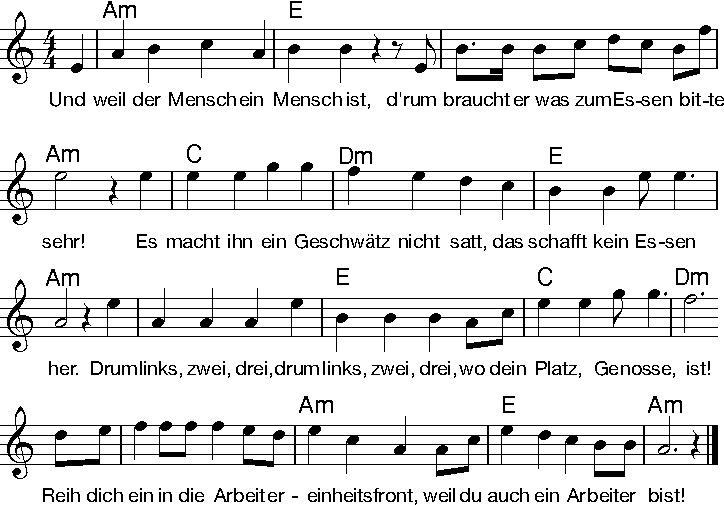
\includegraphics[width=1\textwidth]{Noten/Lied033b.pdf}	

\beginverse
Und \[Am]weil der Mensch ein \[E]Mensch ist,
d'rum braucht er auch Kleider und \[Am]Schuh!
Es \[C] macht ihn ein \[Dm]Geschwätz nicht warm
und \[E]auch kein Trommeln \[Am]dazu.
\endverse

\beginchorus
D'rum \[Am]links, zwei, drei! D'rum \[E]links, zwei, drei!
Wo dein \[C]Platz, Genosse \[Dm]ist!
Reih dich ein in die Arbeiter\[Am]einheitsfront, weil du \[E]auch ein Arbeiter \[Am]bist.
\endchorus

\beginverse
Und ^weil der Mensch ein ^Mensch ist,
d'rum hat er Stiefel im Gesicht nicht ^gern!
Er ^will unter sich ^keinen Sklaven seh'n
und ^über sich keinen ^Herr'n.
\endverse
%\renewcommand{\everychorus}{\textnote{\bf Refrain (wdh.)}}



\beginchorus
D'rum \[Am]links, zwei, drei! D'rum \[E]links, zwei, drei!
Wo dein \[C]Platz, Genosse \[Dm]ist!
Reih dich ein in die Arbeiter\[Am]einheitsfront, weil du \[E]auch ein Arbeiter \[Am]bist.
\endchorus

\beginverse
Und ^weil der Prolet ein ^Prolet ist,
d'rum wird ihn kein anderer be^frei'n!
Es ^kann die Befreiung ^der Arbeiter nur
das ^Werk der Arbeiter ^sein.
\endverse



\beginchorus
D'rum \[Am]links, zwei, drei! D'rum \[E]links, zwei, drei!
Wo dein \[C]Platz, Genosse \[Dm]ist!
Reih dich ein in die Arbeiter\[Am]einheitsfront, weil du \[E]auch ein Arbeiter \[Am]bist.
\endchorus


\endsong

\beginscripture{}
Das Lied entstand Ende 1934 für die Erste Internationale Musikolympiade und wurde 1935 in Straßburg uraufgeführt. Es thematisiert Brechts Überzeugung, nur eine Einheitsfront aus Kommunisten und Sozialdemokraten könne den Nationalsozialismus aufhalten.
\endscripture
